\chapter{Bedingungen für die Existenz von SLTRs}\label{main_theory}

Wir werden in diesem Kapitel hinreichende Bedingungen für die Existenz von SLTRs erarbeiten. Als ersten Schritt wollen wir jedoch eine notwendige Eigenschaft festhalten.

Sei $G$ ein planer intern 3-zusammenhängender Graph mit Aufhängungen $\{a_1,a_2,a_3\}$. Nehmen wir für einen Moment an, dass wir schon eine SLTR für $G$ gefunden haben. Für die Zeichnung müssen die folgenden Bedingungen gelten:

\begin{itemize}
\item Jeder Knoten $v \in V$ hat in maximal einem inzidenten Gebiet $f$ einen flachen Winkel.
\item Jedes Gebiet $f \in F$ (inklusive dem Äusseren) hat genau drei Ecken. Es muss also in jedem Gebiet $|f|-3$ flache Winkel an Knoten geben.
\end{itemize}

Diese Bedingungen liefern eine notwendige Bedingung für die Existent einer SLTR. Sie ist in der nächsten Definition festgehalten.

\begin{definition}[FAA]\label{def_faa}
Sei $G=(V,E,F)$ ein planer Graph. Eine \textit{flache Winkel Zuweisung} $\phi$, kurz \textit{FAA} (nach dem englischen \textit{flat angle assignment}), ist eine partielle Zuordnung der Knoten zu den Gebieten. Es muss gelten:
\begin{itemize}
\item [F1] Jedem Gebiet $f$ sind genau $|f|-3$ Knoten zugewiesen.
\item [F2] Jeder Knoten $v$ ist höchstens einem Gebiet zugewiesen.
\end{itemize}
Für den Fall, dass Aufhängungen gegeben sind, fordern wir zusätzlich:
\begin{itemize}
\item [F3] Die inzidenten Knoten des äusseren Gebietes, die keine Aufhängungen sind, müssen dem äusseren Gebiet zugewiesen sein.
\end{itemize}

\end{definition}

\begin{example}
Links und rechts in Abbildung \ref{exp_faa} sehen wir den selben planaren Graphen $G$ mit zwei unterschiedlichen Zeichnungen. Das äussere Gebiet ist bei beiden das selbe. Die Pfeile stellen hier die Zuweisung der Knoten zu den inneren Gebieten da (also das FAA). Auf der rechten Seite sehen wir eine SLTR von $G$ mit dem passenden FAA. Auf der linken Seite ist ein FAA eingezeichnet, das keine SLTR induziert.

\begin{figure}[h]
	\centering
  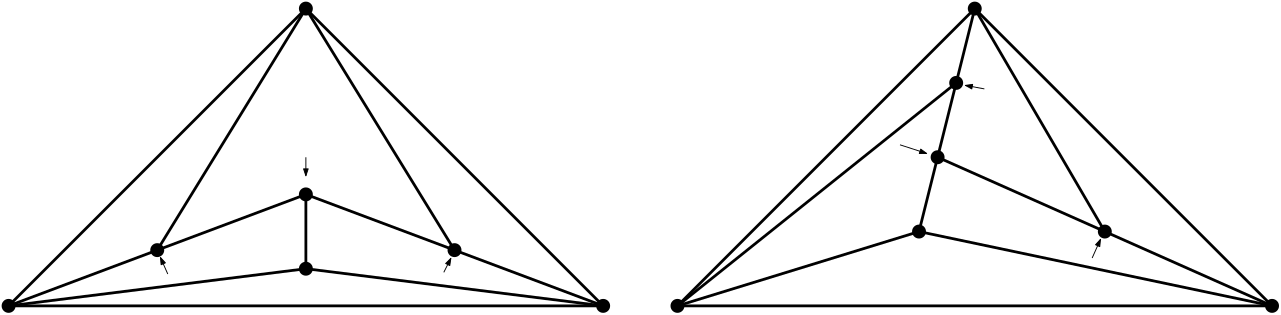
\includegraphics[width=0.9\textwidth]{faa_def.png}
  \caption{Der selbe planare Graph mit zwei FAA, von denen nur das rechte eine SLTR induziert.}
  \label{exp_faa}
\end{figure}
\end{example}

Somit induziert jede SLTR genau ein FAA. Ein planer Graph kann also nur dann eine SLTR besitzen, wenn mindestens ein FAA existiert. Wie in Beispiel \ref{bsp_faa} gezeigt, induziert jedoch nicht jedes FAA eine SLTR. Um hinreichende Bedingungen für SLTRs zu erhalten, werden sich die nächsten beiden Abschnitten mit zwei Ansätzen nach Aerts und Felsner beschäftigen. Der erste Ansatz aus \cite{af13} liefert ein System aus harmonischen Gleichungen aus dessen Lösung eine SLTR folgt. In Teilen darauf basierend, stellt der zweite Ansatz aus \cite{af15} einen Zusammenhang zwischen Schnyder Woods und FAAs her und die Existenz passender Paare impliziert wieder die Existenz von SLTRs.

\section{SLTRs durch harmonische Funktionen}\label{harmonic_approach}

Die Beweise zu den in diesem Kapitel aufgestellten Propositionen und Theoremen werden ausgelassen. Sie befinden sich, wenn nicht anders angegeben, in \cite{af13} . Zum Einstieg eine weitere Definition, die es ermöglicht eine Beobachtung zu SLTRs festzuhalten.

\begin{definition}[Begrenzende Zykel und kombinatorisch konvexe Ecken]\label{def_ccc}
Sei $G$ ein planer Graph mit Aufhängungen $\{a_1,a_2,a_3\}$ und einem FAA $\phi$ von G. Sei $H$ ein zusammenhängender Teilgraph von G und $\gamma=\gamma(H)$, der H umrandende Weg in G. Bei $\gamma$ handelt es sich um die Kanten und Knoten des äusseren Gebiets von H. Knoten und Kanten können mehrfach vorkommen. Wir werden so erhaltene $\gamma$ als \textit{begrenzende Zykel} bezeichnen. $int(\gamma)$ sei die Menge aller Knoten, Kanten und Gebiete aus G die im Inneren von $\gamma$ oder auf $\gamma$ liegen. Einen Knoten $v$ aus $\gamma$ bezeichnen wir als \textit{kombinatorisch konvexe Ecke} von $\gamma$ im Bezug auf $\phi$, falls gilt:
\begin{itemize}
\item [E1] $v$ ist eine Aufhängung, oder
\item [E2] $v$ ist nicht durch $\phi$ zugeordnet und es existiert eine Kante $e = (v,w)$ mit $e \notin int(\gamma)$, oder
\item [E3] $v$ ist einem Gebiet $f$ zugeordnet, $f \notin int(\gamma)$ und es existiert eine Kante $e = (v,w)$, sodass $e \notin int(\gamma)$.
\end{itemize}

\end{definition}

\begin{figure}[h]
	\centering
  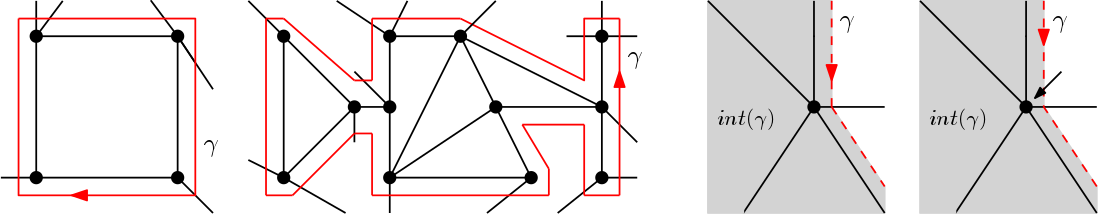
\includegraphics[width=0.9\textwidth]{corner_def.png}
  \caption{Auf der linken Seite zwei Beispiele für \textit{begrenzende Zykel} und rechts für \textit{kombinatorisch konvexe Ecken} mit und ohne zugewiesenem Knoten.}
  \label{corner_def}
\end{figure}

\begin{example}
Betrachten wir eine SLTR und einen begrenzenden Zykel $\gamma$, der nicht von einem Pfad induziert wird. In Abbildung \ref{pic_exp_cycle} ist so eine SLTR mit dem begrenzenden Zykel in rot abgebildet. Sei $K$ die konvexe Hülle von $\gamma$ in der SLTR. Sie ist hier grau unterlegt. Dann muss $K$ mindestens drei Ecken haben an denen der Aussenwinkel grösser als $\pi$ ist (die drei roten Kreise). Es handelt sich um geometrisch konvexe Ecken in der Zeichnung. Nun ist der Knoten $v$ an dieser Ecke entweder eine Aufhängung (wie unten links) oder es muss eine Kante geben die $K$ verlässt, denn in einer SLTR kann kein Winkel (ausser an den Aufhängungen) grösser sein als $\pi$. Wenn der Knoten $v$ an der Ecke keine Aufhängung ist dann existiert also mindestens eine Kante $(v,w) \notin K$. Es handelt sich also bei $v$ auch um eine kombinatorisch konvexe Ecken von $\gamma$. Somit hat $\gamma$ mindestens drei kombinatorisch konvexe Ecken in der SLTR.
\end{example}

\begin{figure}[h]
	\centering
  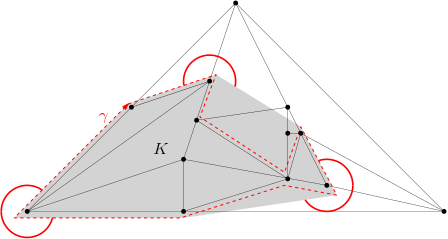
\includegraphics[width=0.7\textwidth]{exp_cycle.png}
  \caption{Eine SLTR eines Graphen mit einem begrenzenden Zykel $\gamma$ in rot. Die roten Kreise stellen drei geometrisch und kombinatorisch konvexe Ecken von $\gamma$ dar.}
  \label{pic_exp_cycle}
\end{figure}

Die Beobachtung aus dem Beispiel gilt allgemein für SLTRs und begrenzende Zykel. Die folgende Präposition nach \cite[Prop 2.2, Prop 2.4]{af13} hält sie fest.

\begin{proposition}\label{com_prop}
Sei $G$ ein planer Graph der eine SLTR zulässt. Sei weiter $\phi$ das von der SLTR induzierte FAA. Sei $H$ ein zusammenhängender Teilgraph von G (kein Pfad) und $\gamma = \gamma(H)$ sein begrenzender Zykel. Falls $v$ eine geometrisch konvexe Ecke von $\gamma$ in der SLTR ist, dann ist $v$ auch eine kombinatorisch konvexe Ecke von $\gamma$ hinsichtlich $\phi$. Somit gilt:
\begin{itemize}
\item [E4] Jeder begrenzende Zykel $\gamma$, der nicht von einem Pfad induziert wird, hat hinsichtlich $\phi$ mindestens drei kombinatorisch konvexe Ecken.
\end{itemize}
\end{proposition}

Proposition \ref{com_prop} liefert also eine notwendige Bedingung damit ein FAA von einer SLTR induziert sein kann. Dies ist sogar eine hinreichende Bedingung, wie im Verlauf des Kapitels in Theorem \ref{com_theo} gezeigt wird. 

\begin{definition}[Gutes-FAA]
Wir nennen ein FAA, das E4 aus Proposition \ref{com_prop} erfüllt, im Weiteren \textit{Gutes-FAA} oder kurz \textit{GFAA}.
\end{definition}

Aerts und Felsner zeigen, dass ein Gutes-FAA eine \textit{Kontaktfamilie von Pseudosegmenten} induziert die \textit{dehnbar} ist und sich somit geradlinig darstellen lässt.

\begin{definition}[Kontaktfamilie von Pseudosegmenten]
Eine \textit{Kontaktfamilie von Pseudosegmenten} ist eine Familie $\Sigma = \{c_i\}_{i\in I}$ von einfachen Kurven $$c_i:[0,1] \to \mathbb{R}^2, \text{ mit } c_i(0) \neq c_i(1),$$ sodass alle Kurven $c_i,c_j$ mit $i \neq j$ maximal einen gemeinsamen Punkt haben. Dieser Punkt muss dann ein Endpunkt von mindestens einer der Kurven sein.
\end{definition}

Ein GFAA $\phi$ liefert eine Relation $\rho$ auf den Kanten von G. Zwei Kanten $(v,w)$ und $(v,u)$, beide adjazent zu $f$, stehen genau dann in Relation, wenn $\phi(v)=f$. $(v,w)$ und $(v,u)$ müssen also auf der selben Seite  des Dreiecks $f$ in der SLTR liegen. Der transitive Abschluss dieser Relation liefert eine Äquivalenzrelation $\rho$. Die Aquivalenzklassen von $\rho$ bilden eine Kontaktfamilie von Pseudosegmenten.

Nennen wir die Äquivalenzklassen von $\rho$ Kurven, dann gilt nach F2, dass jeder Knoten nur einem Gebiet zugeordnet werden kann und somit auch nur im Inneren von einer Kurve liegt. Die Kurven können sich also nicht kreuzen, sondern es kann nur eine an einer anderen enden. Weiter hat jede Kurve unterschiedliche Anfangs- und Endpunkte und kann sich nicht selbst berühren. Dies kann man so begründen, dass sonst der resultierende begrenzende Zykel $\gamma$ nur eine beziehungsweise zwei kombinatorisch konvexe Ecken hätte. Das wäre ein Widerspruch zu E4. Analog können zwei Kurven nicht ihre Anfangs- und Endpunkte teilen, da sonst wieder ein Zykel mit zu wenigen Ecken entstehen würde. Für eine von einem FAA $\phi$ induzierte Kontaktfamilie schreiben wir auch $\Sigma_{\phi}$. 

\begin{figure}[h]
	\centering
  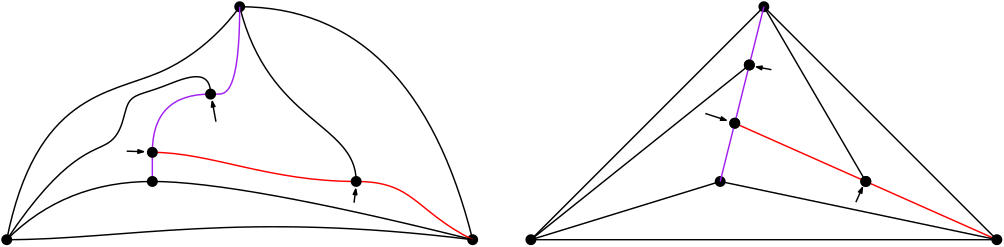
\includegraphics[width=0.95\textwidth]{pseudo_seg.png}
  \caption{Die Kanten von G als Kontaktfamilie von Pseudosegmenten induziert durch die Äquivalenzrelation. In rot und grün die beiden Äquivalenzklassen bzw. Kurven, die mehr als eine Kante beinhalten.}
\end{figure}

\begin{definition}
Sei $\Sigma$ ein Kontaktfamilie von Pseudosegmenten und $S\subseteq\Sigma$. Wir nennen einen Punkt $p\in S$ einen \textit{freien Punkt}, falls er die folgenden Bedingungen erfüllt.
\begin{itemize}
\item p ist ein Endpunkt eines Pseudosegmentes aus S.
\item p liegt nicht im Inneren eines Pseudosegmentes aus S.
\item p liegt am äusseren Rand von S.
\item p ist entweder eine Aufhängung von G oder berührt ein Pseudosegment, welches nicht zu S gehört.
\end{itemize} 
\end{definition}

\begin{figure}[h]
	\centering
  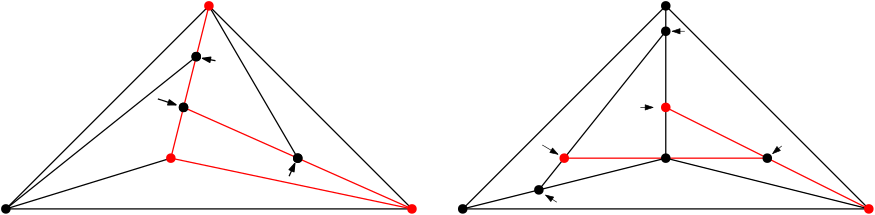
\includegraphics[width=0.95\textwidth]{exp_free.png}
  \caption{Zwei SLTRs mit Teilfamilien von Pseudosegmenten in rot und den freien Punkten dieser Familien ebenfalls in rot.}
\end{figure}

\begin{lemma}\cite[Lemma 2.8]{af13}\label{lemma_af13}
Sei $\phi$ ein Gutes-FAA auf einem planen und intern 3-zusammenhängenden Graphen. Dann gilt: 
\begin{itemize}
\item [E5] Jede Teilmenge $S \subseteq \Sigma_{\phi}$ mit $|S| \geq 2$ hat mindestens 3 freie Punkte.
\end{itemize}
\end{lemma}

Betrachte einen planen, intern 3-zusammenhängenden Graphen $G$ mit Aufhängungen $\{a_1,a_2,a_3\}$ und einem GFAA $\phi$. Wenn die von $\phi$ induzierte Kontaktfamilie $\Sigma_{\phi}$ mit geradlinigen Segmenten darstellbar ist, dann ist diese Darstellung eine zu $\phi$ passende SLTR für $G$. Für den Fall, dass eine solche Darstellung $f:G\to\mathbb{R}^2$ existiert, können für die Koordinaten der Segmente und somit auch der Knoten $v$ von $G$ Gleichungen aufgestellt werden. Die Positionen der Knoten $v$ in der Einbettung $f(v)$ müssen diese Gleichungen erfüllen. Das resultierende Gleichungssystem beinhaltet harmonische Funktionen. Zu diesen folgt ein kurzer Überblick.

\subsection{Harmonische Funktionen auf planaren Graphen}

Die Theorie zu (diskreten) harmonischen Funktionen auf planaren Graphen und ihre Anwendung werden in \cite{lov99} ausführlich behandelt. Es handelt sich um eine Diskretisierung von allgemeinen harmonischen Funktionen, also glatten Funktionen $f:G\subseteq \mathbb{R}^n \to \mathbb{R}$, mit $\Delta f = 0$, wobei $\Delta$ den Laplace Operator beschreibt. Für diese Funktionen gilt, dass der Funktionswert an einem Punkt $x$, dem Durchschnitt der Funktionswerte auf einem Ball um $x$ entspricht. 

Dies führt zu der folgenden Definition im diskreten Fall.

\begin{definition}[Harmonische Funktionen]
Sei $G=(V,E)$ ein planarer zusammenhängender Graph und $S \subseteq V$. Eine Funktion $g:V \to \mathbb{R}$ nennen wir am Knoten $v \in V$ \textit{harmonisch}, falls gilt:
$$ \text{H1} \quad \frac{1}{deg(v)} \sum_{u \in N(v)}(g(u) - g(v)) = 0 \quad \forall v \in V \backslash S \qquad\qquad\qquad\qquad\qquad\qquad\quad\:\,\:$$
Wir können H1 durch das hinzufügen einer nichtnegativen Gewichtsfunktion $\lambda:E\to\mathbb{R}_+$ verallgemeinern. Es gilt $\lambda(v,w) = \lambda_{vw}$.
$$ \text{H2}\quad\frac{1}{deg(v)} \sum_{u \in N(v)}\lambda_{uv}(g(u) - g(v)) = 0 \quad \forall v \in V \backslash S \qquad\qquad\qquad\qquad\qquad\qquad$$
Ein Knoten für den $g$ nicht harmonisch ist, nennt man \textit{Pol}.
\end{definition}

\begin{theorem}\cite[Theorem 3.1.2]{lov99}\label{harmonic_uni}
Für jede nichtleere Teilmenge $S \subseteq V$ und jede Funktion $g_S:S\to\mathbb{R}$ existiert genau eine Funktion $g:V\to\mathbb{R}$, die $g_S$ auf $V$ fortsetzt, sodass $g$ in jedem Knoten $v\in V \backslash S$ harmonisch ist. Wir nennen sie die harmonische Fortsetzung von $g_S$ auf $V$.
\end{theorem}

Ein bekanntes Resultat, dass sich in Form harmonischer Funktionen darstellen lässt, ist Tuttes \textit{rubber-band-representation} aus \cite{tutte63}, die konvexe Zeichnungen für planare Graphen liefert. Man stelle sich einen planaren Graphen vor, bei dem jede Kante durch ein idealisiertes Gummiband\footnote{Die Gummibänder müssen das Hook'sche Gesetzt erfüllen, sodass eine Streckung auf Länge $l$ genau Kraft $l$ benötigt.} ersetzt wird. Fixiere für den Moment alle Knoten in einem beliebigen Punkt. Wähle nun ein äusseres Gebiet und fixiere die Knoten $S\subseteq V$, die in an diesem Gebiet liegen, in zyklischer Reihenfolge und in gleichen Abständen auf einem Kreis um diesen Punkt in der Ebene. Dies definiert $f_S:S \to \mathbb{R}^2$. Wenn wir nun die restlichen Knoten loslassen, dann werden sie von den Bändern in eine neue Position gezogen. Das resultierende Gleichgewicht, das genau dann entsteht, wenn H1 erfüllt ist, entspricht der harmonischen Fortsetzung von $f_S$  auf $V$, wobei $f(v)$ genau der Position von $v$ in der resultierenden Einbettung entspricht und $S$ die Menge der Pole von $f$ ist. Wir können die Kanten zusätzlich noch mit nicht negativen Gewichten $\lambda_{vw}$, versehen um die Einbettung zu verändern. Das folgende Theorem ist das Hauptresultat aus \cite{tutte63}.

\begin{theorem}\label{theo_rubber}
Sei $G$ ein planarer Graph, dann ist eine \textit{Gummiband-Representation (rubber-band-representation)} von $G$ eine planare Einbettung in der Ebene.
\end{theorem}

TODO Bild

\subsection{Das resultierende Gleichungssystem}

Die Theorie zu harmonischen Funktionen lässt sich auf SLTRs anwenden. Sei $G$ ein planarer Graph und $\phi$ ein FAA. Nehme für den Moment an, es existiert eine geradlinige Darstellung der Pseudosegmente $\Sigma_{\phi}$. Wir haben also eine geradlinige Einbettung $f(G)$ der von $\phi$ induzierten Segmente. 

Es gilt für jeden Knoten $v$ im Inneren eines Segmentes, also für jeden zugewiesenen Knoten, dass er auf einer Gerade zwischen seinen beiden benachbarten Knoten $u,w$ auf dem Segment liegen muss. Diese Eigenschaft liefert
\begin{equation}\label{harm_1}
f(v) = \lambda_v f(u) + (1-\lambda_v)f(w) \text{, mit } \lambda_v \in (0,1).
\end{equation}
Für die nicht zugewiesenen Knoten aus $G$ muss in einer SLTR gelten, dass sie sich in der konvexen Hülle ihrer Nachbarn befinden. Wir bilden einen (gewichteten) Schwerpunkt und erhalten
\begin{equation}\label{harm_2}
f(v) = \sum_{u \in N(v)} \lambda_{uv} f(u) \text{, mit }  \sum_{u \in N(v)}\lambda_{uv} = 1 \text{ und } \lambda_{uv} \geq 0.
\end{equation}

Somit erfüllt die so gegebene Funktion $f:V\to\mathbb{R}^2$ mit $f=(f_1,f_2)$ und passend gewählten $\lambda$ wegen (\ref{harm_1}) und (\ref{harm_2}) in beiden Komponenten H2. Es handelt sich somit bei $f_1$ und $f_2$ um harmonische Funktionen, mit den Polen $\{a_1,a_2,a_3\}$. Nach Theorem \ref{harmonic_uni}, existiert für jede den Beschränkungen entsprechende Wahl von $\lambda$ somit genau eine Funktion $f=(f_1,f_2)$, welche die Gleichungen erfüllt.

Dies führt uns zum Hauptresultat aus \cite{af13}:

\begin{theorem}\label{com_theo}
Sei $G$ ein intern 3-zusammenhängender, planarer Graph und $\Sigma$ eine Familie von Pseudosegmenten, induziert von einem FAA, sodass jede Teilfamilie $S \subset \Sigma$ entweder mindestens drei freie Punkte hat, oder maximal ein Element enthält. Die eindeutige Lösung des aus $\Sigma$ folgenden Gleichungssystems ist eine SLTR.
\end{theorem}

\begin{remark}
Dies bedeutet, dass die weiter oben in Lemma \ref{lemma_af13} festgehaltene notwendige Bedingung auch eine hinreichende ist. Falls wir schon ein Gutes-FAA gefunden haben, dann können wir mit Hilfe des obrigen Ansatzes auch eine Einbettung in der Ebene erhalten. Jedoch gibt es Graphen mit exponentiell vielen FAAs wie in Beispiel \ref{bsp_exp_faa} und es dauert polynominell lange, um E4 zu überprüfen. Wir erreichen also auf diesem Weg also keinen schnellen Algorithmus.
\end{remark}
Aerts und Felsner werfen am Ende von \cite{af13} die Frage nach einer guten Wahl von $\lambda$ auf und wie dies die resultierenden Einbettungen beeinflussen kann. Kapitel \ref{the_program} wird einer möglichen Antwort dieser Frage nachgehen.

\begin{figure}
	\centering
  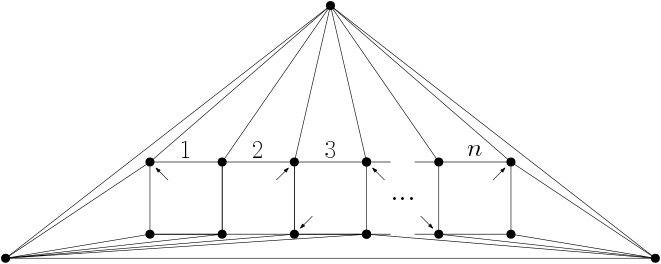
\includegraphics[width=0.6\textwidth]{exp_faa.png}
  \caption{Ein Graph mit exponentiell vielen FAAs.}
  \label{exp_faa}
\end{figure}

\begin{example}\label{bsp_exp_faa}
Betrachten wir eine zusammenhängende Kette von $n$ Quadraten in der Ebene und verbinden wir ihre Eckpunkte mit drei Aufhängungen $a_1,a_2,a_3$, welche ein Dreieck bilden. Der so erzeuge Graph $G$ hat $2n+5$ Knoten und ist in Abbildung \ref{exp_faa} zu sehen. Wir wollen nun ein FAA für diesen Graphen erstellen (welchen nicht zwangsläufig eine SLTR zulässt). Wenn wir von links beginnen und nach rechts laufen können wir in jedem der $n$ inneren Quadrate mindestens aus drei Winkeln auswählen deren Knoten noch nicht zugewiesen sind, um ein FAA zu erstellen. Somit existieren mehr als $3^n$ FAAs für $G.$
\end{example}

\section{Ecken kompatible Paare}

In diesem Abschnitt werden wir uns mit einer zweiten Charakterisierung von SLTRs auf planaren Graphen nach \cite{af15} beschäftigen, die eine Verbindung zwischen Schnyder Woods und FAAs herstellt und so zu einer hinreichenden Bedingung für SLTRs führt. Wir beginnen wieder mit der Definition dieses Zusammenhanges.

\begin{definition}[Ecken Kompatibilität]\label{def_coco}
Ein Paar $(\sigma,\phi)$ aus einem Schnyder Labeling $\sigma$ und einem FAA $\phi$ nenne wir \textit{Ecken kompatibel}, falls:
\begin{itemize}
\item [C1] Das Schnyder Labeling $\sigma$ und das FAA $\phi$ nutzen die selben Aufhängungen.
\item [C2] In jedem inneren Gebiet haben die drei Ecken aus $\phi$ genau drei unterschiedliche Label in $\sigma$.
\end{itemize}
\end{definition}

TODO

\begin{theorem}\label{theo_coco}
Sei G ein planer, intern-3-zusammenhängender Graph mit Aufhängungen. G besitzt eine SLTR, genau dann wenn ein Ecken kompatibles Paar $(\sigma,\phi)$ aus einem Schnyder Labeling $\sigma$ und einem FAA $\phi$ existiert.
\end{theorem}

TODO
